
\def\bl{\mbox{}\newline\mbox{}\newline{}}
\newcommand{\hide}[2]{
\ifthenelse{\equal{#1}{inherited}}%
{}%
{}%
}
\newcommand{\entityintro}[3]{%
\hbox to \hsize{%
\vbox{%
\hbox to .2in{}%
}%
{\bf #1}%
\dotfill\pageref{#2}%
}
\makebox[\hsize]{%
\parbox{.4in}{}%
\parbox[l]{5in}{%
\vspace{1mm}\it%
#3%
\vspace{1mm}%
}%
}%
}
\newcommand{\isep}[0]{%
\setlength{\itemsep}{-.4ex}
}
\newcommand{\sld}[0]{%
\setlength{\topsep}{0em}
\setlength{\partopsep}{0em}
\setlength{\parskip}{0em}
\setlength{\parsep}{-1em}
}
\newcommand{\headref}[3]{%
\ifthenelse{#1 = 1}{%
\addcontentsline{toc}{section}{\hspace{\qquad}\protect\numberline{}{#3}}%
}{}%
\ifthenelse{#1 = 2}{%
\addcontentsline{toc}{subsection}{\hspace{\qquad}\protect\numerline{}{#3}}%
}{}%
\ifthenelse{#1 = 3}{%
\addcontentsline{toc}{subsubsection}{\hspace{\qquad}\protect\numerline{}{#3}}%
}{}%
\label{#3}%
\makebox[\textwidth][l]{#2 #3}%
}%
\newcommand{\membername}[1]{{\it #1}\linebreak}
\newcommand{\divideents}[1]{\vskip -1em\indent\rule{2in}{.5mm}}
\newcommand{\refdefined}[1]{
\expandafter\ifx\csname r@#1\endcsname\relax
\relax\else
{$($ in \ref{#1}, page \pageref{#1}$)$}
\fi}
\newcommand{\startsection}[4]{
\gdef\classname{#2}
\subsection{\label{#3}{\bf {\sc #1} #2}}{
\rule[1em]{\hsize}{4pt}\vskip -1em
\vskip .1in 
#4
}%
}
\newcommand{\startsubsubsection}[2]{
\subsubsection{\sc #1}{%
\rule[1em]{\hsize}{2pt}%
#2}
}
\date{\today}
\pagestyle{myheadings}
\oddsidemargin 0in
\evensidemargin 0in
% \topmargin -.8in
\chardef\bslash=`\\
\textheight 9.4in

\chapter{Proof Builder}

\section{User interface}

Donald Norman's research on UI was used.
Typical Android application conventions such were followed such as the use and look if dialog boxes. Also the dark background with light font is very common for this platform.

Perceived affordances as described by Norman were implemented in regards to touch screen buttons that users will press and lists that users can push up or down.

In accordance with the project procedure the first part of the proof builder to be designed was the user interface. The user interface was developed by taking simple user stories that described what a user would want to do and attempting to create a graphical interface for each task that would be intuitive to use.

\subsection{Proof thingy}
It was decided that displaying the actual proof was the most important part of the user interface and that this would be given the majority of the screen space. Since space is limited on mobile devices, it was decided that the application would display in landscape mode to enable most sentences of FOL to fit onto one line, enhancing the readability of the proof. The intent was that the proof would resemble a hand written proof of FOL as much as possible. 

This proof section of the screen will start off empty and each line will be displayed as it is added to the proof.

In order from left to right each line displays the following:
\begin{itemize}
\item{The line number of the proof.}
\item{A boxed variable if one has been introduced in this line. }
\item{The FOL sentence , this may be blank if a variable is introduced without an assumption.}
\item{The justification of this line.}
\end{itemize}
When more more lines are added than can fit on the screen then the list of lines becomes vertically scrollable. The user may scroll the list by simply using their finger to push the list up and down. This is an intuitive motion which all users who tested the product used without prompting.

\begin{figure}[h!]
\centering
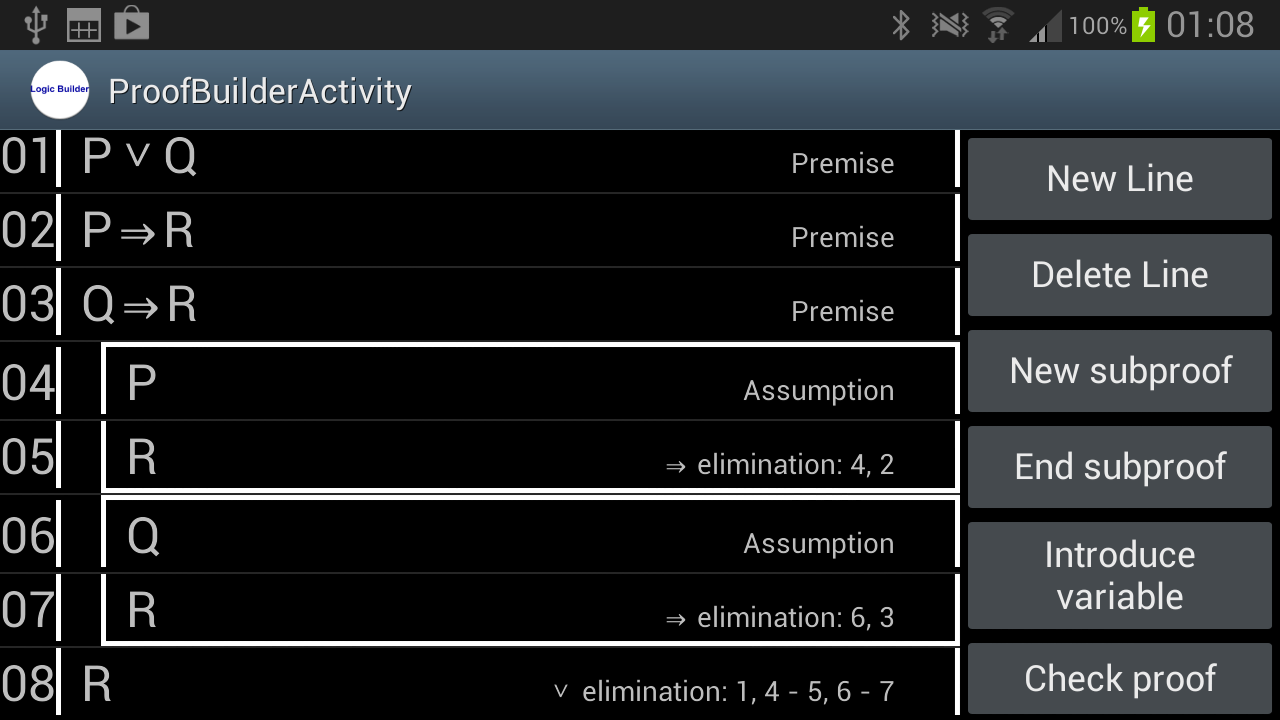
\includegraphics[width=0.9\textwidth]{Images/sampleproof.png}
\caption{User interface for proof builder}
\label{fig:Compilation}
\end{figure}

\FloatBarrier




\subsection{Button bar}

A section fixed to the right hand side displays a button bar which allows the user to carry out various tasks. The buttons make use of the proximity and similarity to give the user the sense that the buttons are a group of objects, rather than separate entities. 

The buttons are listed below along with a description of how the graphical user interface reacts and changes for each.

\subsubsection{New line}

Selecting the new line button will activate the formula checker activity. This will appear as described in the previous chapter. After the user submits a sentence a new line is added to the end of the proof  with the same indentation as the previous line and within any boxes that the previous line was inside of. The justification of the line will be set to `No justification given'. This serves as a prompt to the user to add a justification,


\subsubsection*{Delete line}

Pressing the delete line button will remove the most recent line of the proof.

\subsubsection*{New subproof}
When the new subproof button is pressed the formula checker activity will be displayed. Upon submitting a sentence a new line will be added  to the end of the proof which is indented more than the previous line and the top section of a box will surround it. The justification for this line is set to `Assumption'.
\subsubsection*{End subproof}
Similarly, pressing the option end subproof will present the user with the formula checker activity to enter a sentence. When a sentence has successfully been submitted the new line will be added at the end of the proof. Additionally the bottom part of the box will be formed and the whole subproof will be neatly enclosed within the box. As with the new line button the justification for this line is set to `No justification given'.

\subsubsection*{Introduce variable}

Choosing the introduce variable option will display a dialog box. The user will be able to use this dialog box to name a variable that is to be introduced to the proof. Should the user enter a variable name that is not valid such as an empty name then a message will be displayed informing them why the name cannot be accepted and they will then be given the opportunity to enter a different name.


A checkbox also appears within the dialog box. The user may mark the checkbox if they wish to make an assumption as well as introduce a variable. After an appropriate name has been chosen and the user chooses the OK button, the formula checker activity will be displayed  if the user has marked the checkbox. Once the user has submitted or sentence, or if the checkbox was not marked, then line will be added to the end of the proof.

The variable will be displayed in a small box. If a sentence was submitted this will be displayed followed by the justification which will be set to the word `Assumption'. Otherwise, the rest of the line will be left empty. Similar to starting subproof, the whole line is indented more than the previous and the top section of a box will surround it.


\subsubsection*{Check proof}

Pressing check proof triggers the display of a dialog box. This dialog box will inform the user whether the proof entered so far is complete and valid. If not it will inform the user as to why with messages such as `All subproofs must be closed to check proof' or `Line x has not been justified', where x is the number of a line of which no justification has been specified. If the proof is complete and valid then the user will presented with a message that confirms that the premises semantically entails the conclusion e.g for premises $\phi_1, \hdots , \phi_n$ and conclusion $\psi$ the message would read `Congratulations,  you have successfully proved: $\phi_1, \hdots , \phi_n \models \psi$'                                                                                                                                                                                  


\subsection{Justifying a line}

To change the justification of a line in the proof the user simply needs to touch the line that they wish to change. This will bring up a dialog box. A drop-down list contains all the rules of inference. The display will change depending on which ROI is currently selected. The labels serve as clues to what form the premises take for this ROI. 

A drop-down list is displayed next to the label for each premise which can be used to specify which line or subproof is to be used.  The drop-down list will only contain single line numbers, if the premise requires just a sentence, or a block of line numbers, if this premise needs to be a subproof. Furthermore, only line numbers and whole subproofs that occur after the line being justified appear in the list. 

When the user has specified ROI to use and the premises then the OK button must be pressed to continue. If there is a problem with the justification an error message is displayed which explains why it has not been accepted. This is explained further in section 4.3. If the justificationis accpeted then dialog box is removed and the justification of the chosen line is updated with the chosen ROI and the line numbers of the premises used.

As can be seen in figure 4.2 the proof is partially visible when justifying a line. The system was designed this way as when it was not visible users commented that they found it difficult to remember the lines numbers that were to be used as premises for the ROI. Having the proof visible even if partially greatly helped users to identify the correct line numbers that they needed.

	
\begin{figure}[h!]
\centering
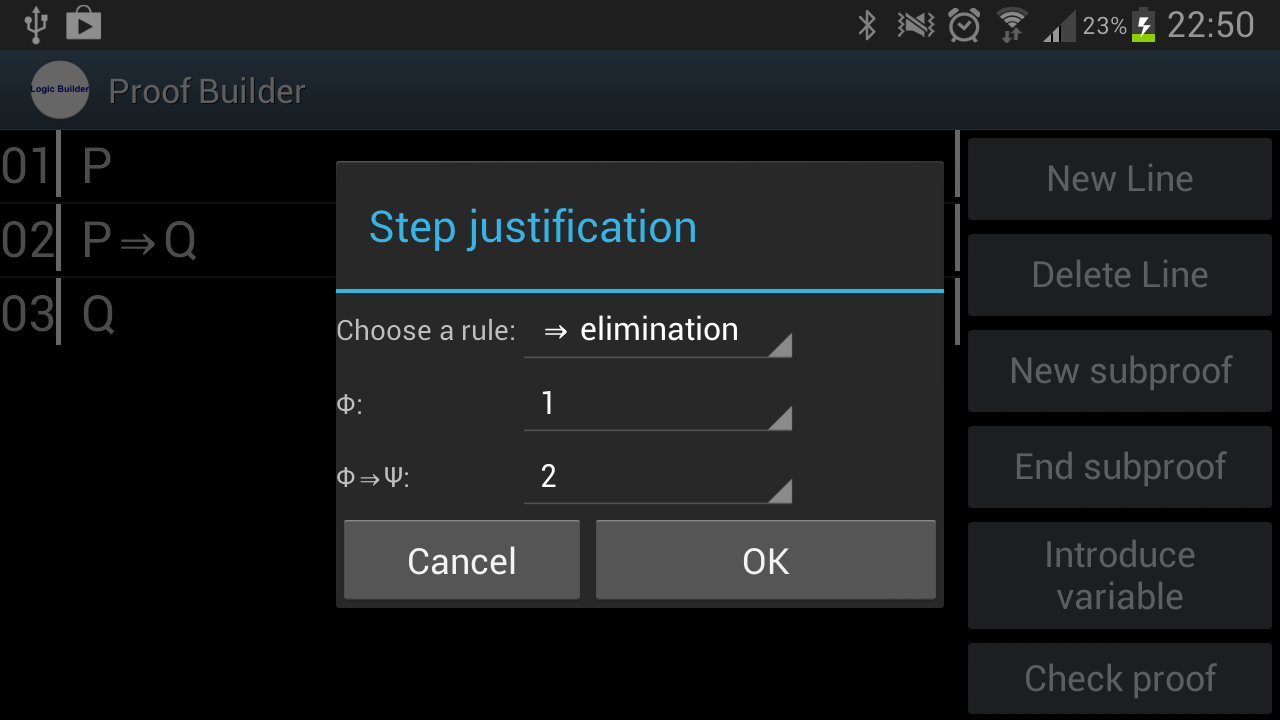
\includegraphics[width=0.9\textwidth]{Images/justification.png}
\caption{User interface for justifying a line}
\label{fig:Compilation}
\end{figure}

\FloatBarrier


\section{Rules of Inference}

Rules of inference were programmed in the Java language. A method was created for every ROI. This method then takes as arguments the premises of each rule followed by the line that is being justified. The order of the premises that are passed into the method must be the same as defined by the ROI. 

As mentioned in the previous section, sentences of FOL are stored in a tree data structure. This is utilised by the rules of inference since all data about about a sentence can be found from only the root node. If a premise is single statement then the root node of the statement should be passed into the method. If a premise is a sub-proof then a list of root nodes should be passed. This list may contain either the whole subproof or only the required parts such as the first and last line. The order of nodes must be the same as the order of the lines in the subproof.  

Firstly, each method will check that the premises and the conclusion are of all of the correct form for this ROI. The correct form may be any WFF of FOL or it may be more restrictive such as it has to be a negation of a sentence. If any of the arguments do not match the expected form then an exception is thrown by the method. There are two types of exception that can be thrown: PremiseException and ConclusionException. Intuitively these exceptions relate to the premises or conclusion not being of the required form. Each exception contains a message explaining what the discrepancies between the given arguments and what would be expected.

In most cases, to check whether a sentence is of the correct form only requires looking at the operator with greatest scope. This is handled efficiently by the tree structure since only the root node has to be inspected. Furthermore, finding part of a sentence, such as the LHS  or RHS of a binary operator, is also very simple with the tree data structure. This is done by taking the appropriate child node of the operator; this child will be the root node of the sub tree for the part of the sentence required.

Subsequently, the method will then evaluate the ROI on the given premises. If only one conclusion is possible, such as the case of $\land$ introduction, then this unique conclusion is determined and compared with the line that is being justified. If they are not syntactically equivalent then a ConlusionException is thrown. This exception contains an error message that details what would have been expected using the chosen ROI on the given arguments. If more than one conclusion is possible then the line that is being justified is checked to make sure that it is a possible conclusion using the chosen ROI and the given premises.

\subsection{API} 

The ROI have been coded as a standalone component that may be used by other applications. As such an API has been created that explains how the ROI class can be used. Full technical documentation can be found in the appendix. 

Documentation was generated using Javadocs. 
The API contains:
\begin{itemize}
\item{A brief description to describe the purpose of the class.}
\item{All publicly accessible fields of the class, along with a description.}
\item{For each method the API may contain:}
\begin{itemize}
\item{A description of the purpose of the method}
\item{The name, type and a description of each parameter}
\item{The type and description of  what is returned by the method}
\end{itemize}
\end{itemize}

Each rule that deduces a unique conclusion from a set of premises, has two similar and related methods. The methods differ in that one method requires a conclusion given as an argument  and the other does not. The method which does not take a conclusion will return the unique conclusion that is deduced from the premises. 

Below is an example of how the API represents such a case, using overloaded methods: 


$\\$
\begin{itemize}

\item{\vskip -1.9ex 
\membername{doubleNegationElimination}
{\tt public static SimpleNode {\bf doubleNegationElimination}( {\tt \\ logic.proof.builder.parser.SimpleNode } {\bf p} )
\label{l41}\label{l42}}%end signature
\begin{itemize}
\sld
\item{
\sld
{\bf Parameters}
\sld\isep
\begin{itemize}
\sld\isep
\item{
\sld
{\tt p} - The root node of a sentence of FOL starting with two negations}
\end{itemize}
}%end item
\item{{\bf Returns} - 
The premise without the first two negations 
}%end item
\item{{\bf Exceptions}
\begin{itemize}
\sld
\item{\vskip -.6ex{\tt logic.proof.builder.exceptions.PremiseException} - If premises are not of the correct form for this rule}
\end{itemize}
}%end item
\end{itemize}
}%end item
\divideents{doubleNegationElimination}
\item{\vskip -1.9ex 
\membername{doubleNegationElimination}
{\tt public static void {\bf doubleNegationElimination}( {\tt \\ logic.proof.builder.parser.SimpleNode } {\bf p},
{\tt logic.proof.builder.parser.SimpleNode } {\bf conclusion} )
\label{l43}\label{l44}}%end signature
\begin{itemize}
\sld
\item{
\sld
{\bf Parameters}
\sld\isep
\begin{itemize}
\sld\isep
\item{
\sld
{\tt premise} - The root node of a sentence of FOL starting with two negations}
\item{
\sld
{\tt conclusion} - The root node of the sentence being justified}
\end{itemize}
}%end item
\item{{\bf Exceptions}
\begin{itemize}
\sld
\item{\vskip -.6ex{\tt logic.proof.builder.exceptions.ConclusionException} - If conclusion does not follow from using rule on given
arguments}
\item{\vskip -.6ex{\tt logic.proof.builder.exceptions.PremiseException} - If premises are not of the correct form for this rule}
\end{itemize}
}%end item
\end{itemize}
}%end item
\divideents{doubleNegationIntroduction}

\end{itemize}





\section{Proof structure}

When the application is started an Java Proof object is instantiated. This object stores data about the proof and is used t

The Proof object is a high level abstraction that hides the complexity of the actual proof structure. A proof consists of a tree of ProofSteps. Each ProofStep contains data about a particular line of proof. This data includes:
\begin {description}
\item[lineNumber] The number of the line in the proof
\item[rootNode] Root node of the sentence tree
\item[subproofs] List of pointers to sub proofs following this line
\item[next] Pointer to next non subproof step
\item[parent] Pointer to previous step
\item[introducedVariable] The name of the introduced variable, null if n/a
\item[level] The number of nested subproofs that this line is inside of
\item[justification] The ROI used along with line numbers of the premises
\end{description}

 
A crucial part of Fitch style proofs is the use of subproofs and the notion of scope. Scope, in this context, is the notion that a line within a subproof cannot be used as a premise of a ROI for any line outside of the subproof. As well as this the premises used for a ROI must precede the line being justified.  Since each ProofStep explicitly stores pointers to other steps and subproofs, the information which other lines or subproofs can be used as a premises to justify this line can be found quickly, without having to traverse the whole proof tree.


\startsection{Class}{Proof}{l0}{%
{\small Stores all data necessary to construct a proof. Simple Methods are provided to manipulate
the proof such as adding or deleting lines.}
\vskip .1in 
\startsubsubsection{Declaration}{
\fbox{\vbox{
\hbox{\vbox{\small public 
class 
Proof}}
\noindent\hbox{\vbox{{\bf extends} java.lang.Object}}
}}}
\startsubsubsection{Fields}{
\begin{itemize}
\item{
public List predicates\begin{itemize}\item{\vskip -.9ex A list of all the named predicates in the proof. Used to populate the
predicate list.}\end{itemize}
}
\end{itemize}
}
\startsubsubsection{Constructors}{
\vskip -2em
\begin{itemize}
\item{\vskip -1.9ex 
\membername{Proof}
{\tt public {\bf Proof}( )
\label{l3}\label{l4}}%end signature
\begin{itemize}
\sld
\item{
\sld
{\bf Usage}
\begin{itemize}\isep
\item{
Default constructor. Constructs an empty proof
}%end item
\end{itemize}
}
\end{itemize}
}%end item
\end{itemize}
}
\startsubsubsection{Methods}{
\vskip -2em
\begin{itemize}
\item{\vskip -1.9ex 
\membername{addStepAsEndOfSubproof}
{\tt public ProofStep {\bf addStepAsEndOfSubproof}( {\tt logic.proof.builder.parser.SimpleNode } {\bf node},
{\tt java.lang.String } {\bf formula} )
\label{l5}\label{l6}}%end signature
\begin{itemize}
\sld
\item{
\sld
{\bf Usage}
\begin{itemize}\isep
\item{
Adds a new proofstep that is the last line of a subproof
}%end item
\end{itemize}
}
\item{
\sld
{\bf Parameters}
\sld\isep
\begin{itemize}
\sld\isep
\item{
\sld
{\tt node} - Root node of the sentence of the proofstep}
\item{
\sld
{\tt formula} - String representation of the sentence}
\end{itemize}
}%end item
\item{{\bf Returns} - 
Returns the proofstep that has been added 
}%end item
\end{itemize}
}%end item
\divideents{addStepAsNewLine}
\item{\vskip -1.9ex 
\membername{addStepAsNewLine}
{\tt public ProofStep {\bf addStepAsNewLine}( {\tt logic.proof.builder.parser.SimpleNode } {\bf node},
{\tt java.lang.String } {\bf formula} )
\label{l7}\label{l8}}%end signature
\begin{itemize}
\sld
\item{
\sld
{\bf Usage}
\begin{itemize}\isep
\item{
The default method to add a new proofstep to the proof
}%end item
\end{itemize}
}
\item{
\sld
{\bf Parameters}
\sld\isep
\begin{itemize}
\sld\isep
\item{
\sld
{\tt node} - Root node of the sentence of the proofstep}
\item{
\sld
{\tt formula} - String representation of the sentence}
\end{itemize}
}%end item
\item{{\bf Returns} - 
Returns the proofstep that has been added 
}%end item
\end{itemize}
}%end item
\divideents{addStepAsStartOfSubproof}
\item{\vskip -1.9ex 
\membername{addStepAsStartOfSubproof}
{\tt public ProofStep {\bf addStepAsStartOfSubproof}( {\tt logic.proof.builder.parser.SimpleNode } {\bf node},
{\tt java.lang.String } {\bf formula} )
\label{l9}\label{l10}}%end signature
\begin{itemize}
\sld
\item{
\sld
{\bf Usage}
\begin{itemize}\isep
\item{
Adds a new proofstep that is the start of a subproof
}%end item
\end{itemize}
}
\item{
\sld
{\bf Parameters}
\sld\isep
\begin{itemize}
\sld\isep
\item{
\sld
{\tt node} - Root node of the sentence of the proofstep}
\item{
\sld
{\tt formula} - String representation of the sentence}
\end{itemize}
}%end item
\item{{\bf Returns} - 
Returns the proofstep that has been added 
}%end item
\end{itemize}
}%end item
\divideents{addVar}
\item{\vskip -1.9ex 
\membername{addVar}
{\tt public ProofStep {\bf addVar}( {\tt java.lang.String } {\bf var} )
\label{l11}\label{l12}}%end signature
\begin{itemize}
\sld
\item{
\sld
{\bf Usage}
\begin{itemize}\isep
\item{
Add a new proofstep which introduces a boxed variable
}%end item
\end{itemize}
}
\item{
\sld
{\bf Parameters}
\sld\isep
\begin{itemize}
\sld\isep
\item{
\sld
{\tt var} - The name of the variable being introduced}
\end{itemize}	
}%end item
\item{{\bf Returns} - 
Returns the proofstep that has been added 
}%end item
\end{itemize}
}%end item
\divideents{addVar}
\item{\vskip -1.9ex 
\membername{addVar}
{\tt public ProofStep {\bf addVar}( {\tt java.lang.String } {\bf introducedVariable},
{\tt logic.proof.builder.parser.SimpleNode } {\bf rootNode},
{\tt java.lang.String } {\bf formula} )
\label{l13}\label{l14}}%end signature
\begin{itemize}
\sld
\item{
\sld
{\bf Usage}
\begin{itemize}\isep
\item{
Add a new proofstep which introduces a boxed variable alongside an
assumption
}%end item
\end{itemize}
}
\item{
\sld
{\bf Parameters}
\sld\isep
\begin{itemize}
\sld\isep
\item{
\sld
{\tt introducedVariable} - The name of the variable being introduced}
\item{
\sld
{\tt node} - Root node of the sentence}
\item{
\sld
{\tt formula} - String representation of the sentence}
\end{itemize}
}%end item
\item{{\bf Returns} - 
Returns the proofstep that has been added 
}%end item
\end{itemize}
}%end item
\divideents{getCurrentLevel}
\item{\vskip -1.9ex 
\membername{getCurrentLevel}
{\tt public int {\bf getCurrentLevel}( )
\label{l15}\label{l16}}%end signature
\begin{itemize}
\sld
\item{
\sld
{\bf Usage}
\begin{itemize}\isep
\item{
Returns the number of subproofs currently open
}%end item
\end{itemize}
}
\item{{\bf Returns} - 
the number of subproofs currently open 
}%end item
\end{itemize}
}%end item
\divideents{getLines}
\item{\vskip -1.9ex 
\membername{getLines}
{\tt public ArrayList {\bf getLines}( )
\label{l17}\label{l18}}%end signature
\begin{itemize}
\sld
\item{
\sld
{\bf Usage}
\begin{itemize}\isep
\item{
Returns the ordered list of proofsteps
}%end item
\end{itemize}
}
\item{{\bf Returns} - 
the ordered list of proofsteps 
}%end item
\end{itemize}
}%end item
\divideents{removeStep}
\item{\vskip -1.9ex 
\membername{removeStep}
{\tt public void {\bf removeStep}( )
\label{l19}\label{l20}}%end signature
\begin{itemize}
\sld
\item{
\sld
{\bf Usage}
\begin{itemize}\isep
\item{
Removes the most recent line from the proof
}%end item
\end{itemize}
}
\end{itemize}
}%end item
\end{itemize}
}
}
